\chapter{Object Tracking}
To improve the user experience, object tracking was tried. This infers that the application would keep track on where certain objects are on the screen. The thought behind this idea was that the application would not have to constantly run the current frame through YOLO model in order to keep track of where objects were, which could lead to a choppy user experience.

This chapter will describe the concept of object tracking, how it was implemented and tested, as well as our reasoning for not keeping this functionality in the final application.

\section{Testing Object Tracking with Vision package}
Vision is a package from Apple which contains a lot of different methods for images and 
video. It contains still image analysis, image sequence analysis, object tracking, face 
detection etc.

On their website, Apple has a project that lets any user try out the object tracking on a 
video \cite{ObjectTracking}. When trying this on one of the furniture we are going to assemble, the result was 
very promising. While the parts were laying on the floor and simultaneously moving the 
camera around, the objects were tracked fairly well. It was only when the camera was moved 
in such a way that made the pieces rotate in the picture that it started having a hard time 
tracking it.

For solving this, object detection can be performed in a reasonable time interval and be tracked until object detection is performed once again etc.

The difference for this project and Apple's test project is that object tracking is going to 
be performed in real-time. This puts a limit on how many frames per second we can perform 
object tracking, since in a video playback you can just choose how fast you want to feed the 
new images. In real-time, the world doesn't stop moving.

After the system was implemented into our application different frame rates were tested. The 
optimal value was somewhere in-between 10-30 fps. If you went higher than that the 
application would become very choppy and eventually shut down.

Going lower than 10 fps the user will start to experience that the objects are hard to track 
in rapid movements.

For this application, however, the user is not going to encounter any scenarios where 
objects are flying around rapidly. Therefore we will settle for 20 fps as the optimal value 
for performance since any higher amounts don't really contribute to a better experience.

The following lines of code show how the object tracking was set up. One important thing to realize when setting this up is that the heavy calculations are run on a different thread than the main thread (in this case the work thread). 

That is why they can be executed in a while true loop. Later though, when drawing on the GUI wants to be made, they must be done on the main thread.

\begin{lstlisting}[language=swift]
// Project path:
// master-thesis/Application/ObjectDetectionInAR/Assembler/ObjectTracker.swift

func track()
    {
    // Init all variables
        cancelTracking = false
        var trackingObservations = [UUID: VNDetectedObjectObservation]()
        var trackedObjects = [UUID: ObjectRectangle]()
        let requestHandler = VNSequenceRequestHandler()
        let boundingFrame = delegate?.getBoundingFrame()
        
        // Add the objects to track to the created lists above
        for object in objectsToTrack
        {
            let observation = VNDetectedObjectObservation(boundingBox: object.getNormalizedRect(frame: viewFrame))
            trackingObservations[observation.uuid] = observation
            trackedObjects[observation.uuid] = object
        }
        
        // Loop over until a cancel tracking request is made
        while true
        {
            if cancelTracking { break }
            
            var rects = [ObjectRectangle]()
            var trackingRequests = [VNRequest]()
            
            guard let frame = delegate?.getFrame() else {
                usleep(useconds_t(millisecondsPerFrame * 1000))
                continue
            }
            
            for trackingObservation in trackingObservations
            {
                // Create the requests
                let request = VNTrackObjectRequest(detectedObjectObservation: trackingObservation.value)
                request.trackingLevel = .fast
                trackingRequests.append(request)
            }

		   // Perform the requests
            try? requestHandler.perform(trackingRequests, on: frame, orientation: CGImagePropertyOrientation.up)

            for processedRequest in trackingRequests
            {
                // Handle the results from the requests
                guard let observation = processedRequest.results?.first as? VNDetectedObjectObservation else { continue }
                
                if observation.confidence > confidenceThreshold
                {
                    guard let object = trackedObjects[observation.uuid] else { continue }
                   // Set new bounding box
                    object.setNewBoundingBox(newBoundingBox: observation.boundingBox, frame: boundingFrame)
                    trackedObjects[observation.uuid] = object
                    trackingObservations[observation.uuid] = observation
                    
                    rects.append(object)
                }
            }

            DispatchQueue.main.async {
                rects = rects.sorted { $0.name! < $1.name! }
                self.delegate?.trackedRects(rects: rects)
            }
            
            // The tracking will stop if no observation has a high confidence value
            if rects.isEmpty
            {
                DispatchQueue.main.async {
                    self.requestCancelTracking()
                    self.delegate?.trackingLost()
                }
            }

            usleep(useconds_t(millisecondsPerFrame * 1000))
        }
        
        DispatchQueue.main.async {
            self.delegate?.trackingDidStop()
        }
    }
\end{lstlisting}


\section{Combining Object detection with Object Tracking}
The purpose of having the object tracker is to be able to avoid performing object detection and object recognition 30 frames per second or so. Also, doing this with YOLO nets have shown choppy results where an object can be identified in one frame, not identified in the next and then again identified.
There is no real issue with this since both solutions perform really well overall. There is however concerns for the end user to have a good experience.

One way to solve this is to perform the detection and recognition once, to later continue to track the position of those items with a cheaper algorithm.
Object detection and recognition will then be repeated, but only update the state of the rectangles if the correct objects are identified.
In this application, an arrow was drawn between the objects with an instructional text for the user. Doing this created a rather big issue though.

\begin{figure}[!hbtp]
\begin{center}
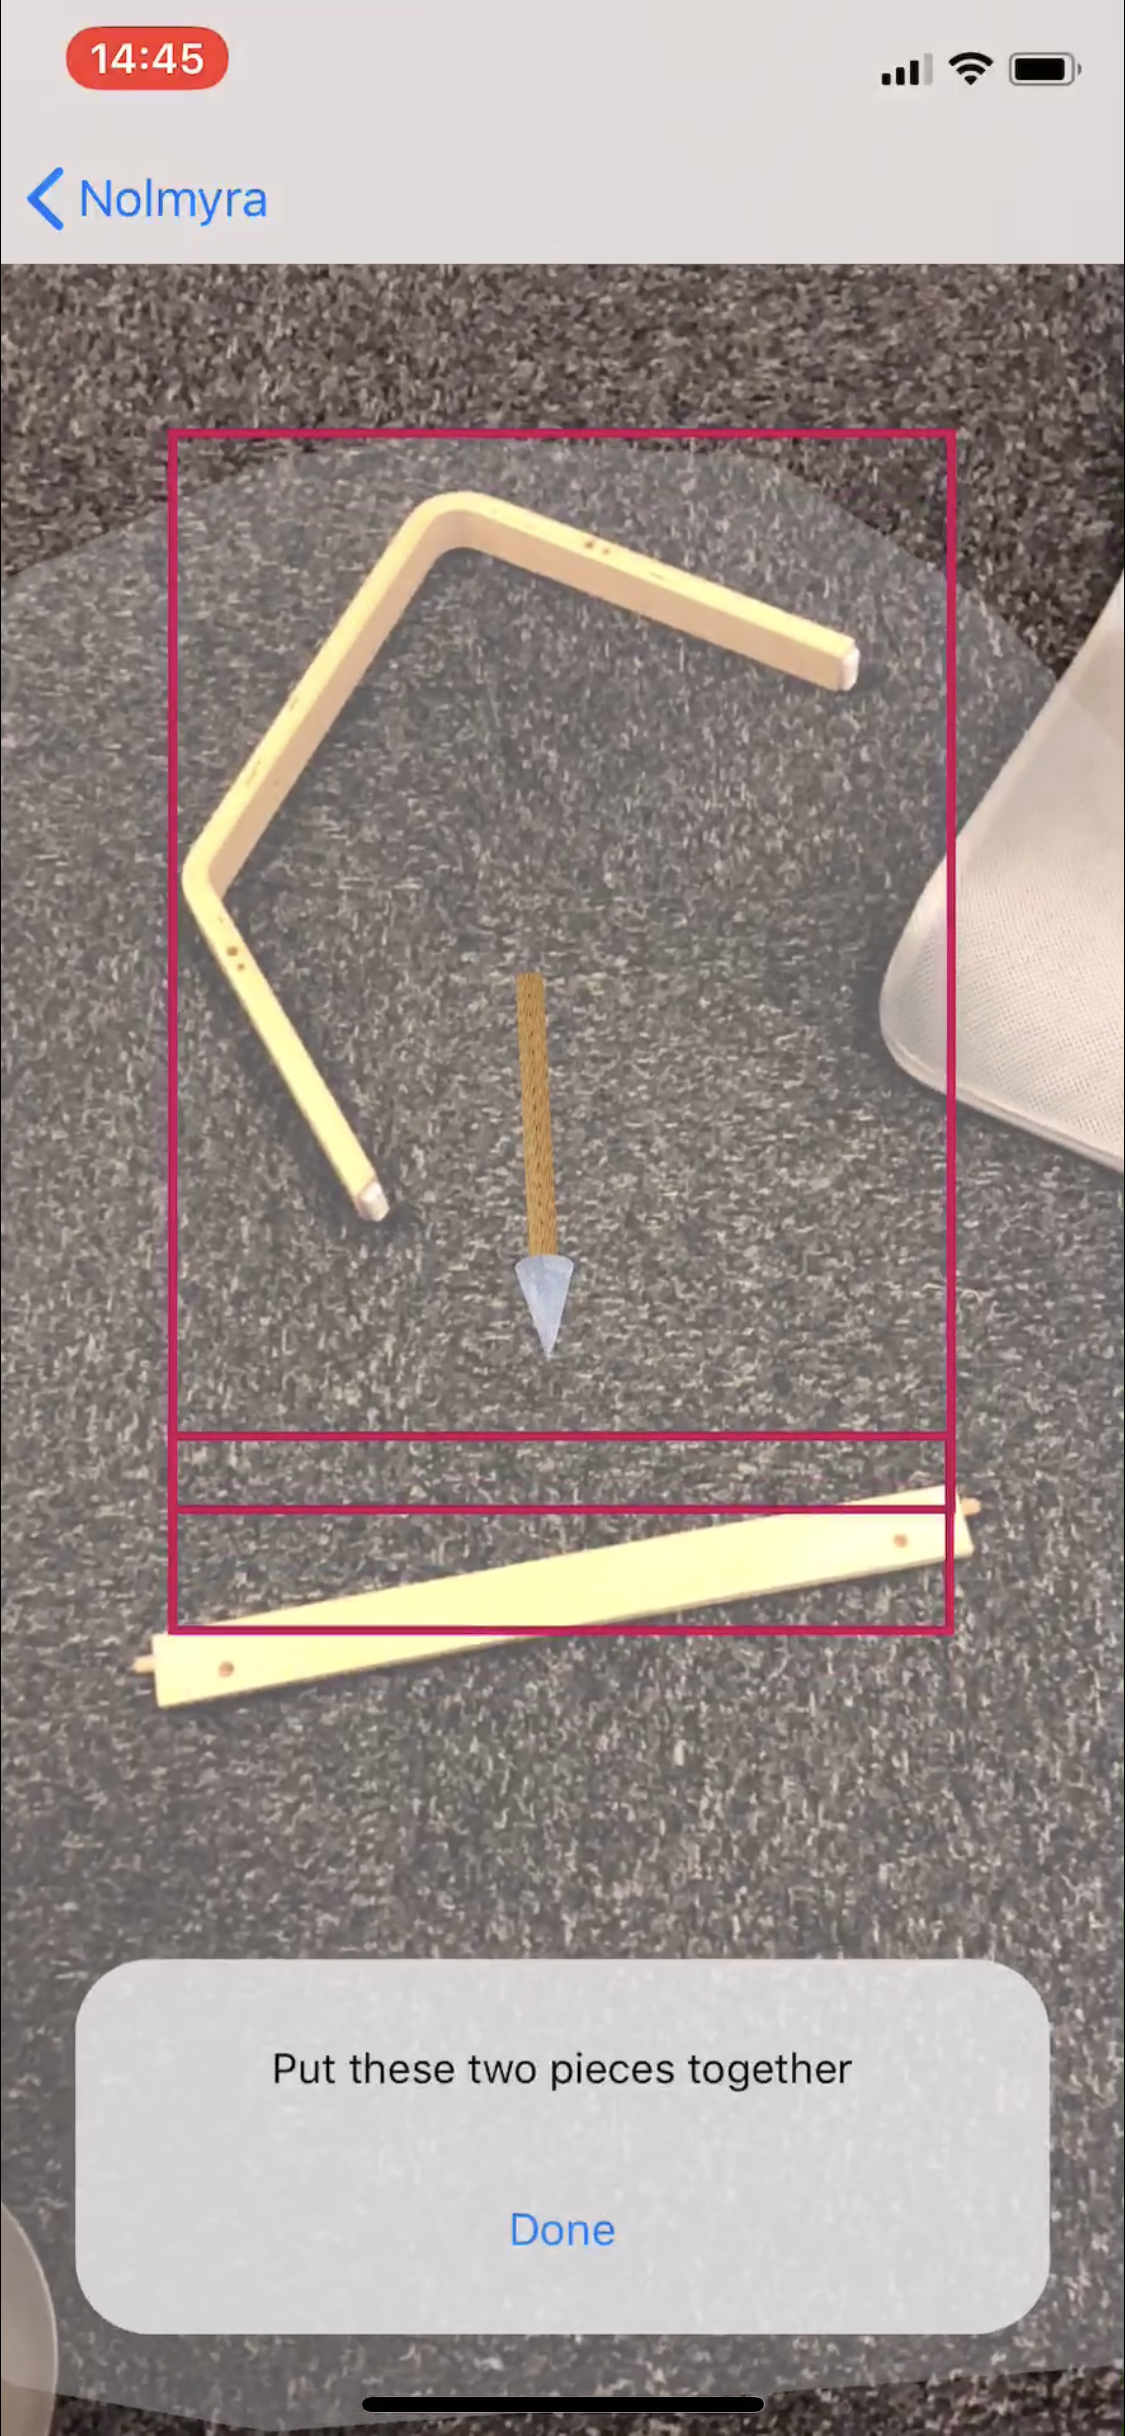
\includegraphics[width = 0.35\textwidth]{./Images/tracking.png}
\caption{The image shows an early stage of the application were two pieces have been recognized by the network and an outline around them has been drawn. Between them, an arrow is rendered on the floor, showing how to put together the two pieces. The objects are continuously being tracked within the frame and the arrow is also updated.}
\label{fig:tracking}
\end{center}
\end{figure}

In this project, ARKit by Apple has been utilized. As previously stated, when working with ARKit, a frame from the camera is fetched by either calling the function snapshot() on the ARSCNView object or getting the currentFrame attribute from the ARSession.
However, both of these images contain both the image from the camera as well as all the virtual items rendered in the ARScene. We did not find a way to capture just the image from  the camera.

This whole scenario created a kind of positive feedback loop because the virtual arrow that was rendered between the objects was usually contained within either one of the tracking rectangles. Thus, the arrow's position was determined by the tracking rectangle and the tracking rectangle was tracking the position of the arrow.
Just the tiniest change in the picture made the arrow jump up and down until it finally got out of frame.

The takeaway from this was to skip object tracking and solve the problem in another way.

An assumption was made that just as talked about before, the furniture parts are laying still on the ground while the user is using the application. That means that we can rely on ARKit to keep track of where the object is for us instead.

Switching gear to that solution made the whole application much better and easier to code. A takeaway from that is that adding more technology to a project does not always equal a better product. Sometimes it is better to use the components the way they are meant to be used and try not to make it more complicated than it needs to be.

\newpage